% ============================================================
% 讲义 — 人教版高一必修2 第6章 平面向量
% 编译命令：xelatex -interaction=nonstopmode 文件名.tex
% ============================================================
\documentclass[12pt, a4paper]{ctexart}
\usepackage[margin=2.2cm]{geometry}
\usepackage{amsmath, amssymb}
\usepackage{enumitem}
\usepackage{tcolorbox}
\usepackage{booktabs}
\usepackage{array}
\usepackage{fancyhdr}
\usepackage{xcolor}
\usepackage{tikz}
\usepackage{hyperref}
\usepackage{graphicx}
\usepackage{multirow}
\usepackage{pgfplots}
\pgfplotsset{compat=1.18}
\usetikzlibrary{calc,arrows.meta,angles,quotes}

% 颜色定义
\definecolor{mainblue}{RGB}{41, 98, 168}
\definecolor{lightblue}{RGB}{230, 240, 255}
\definecolor{tipgreen}{RGB}{34, 139, 87}
\definecolor{lightgreen}{RGB}{235, 250, 240}
\definecolor{warnred}{RGB}{200, 50, 50}
\definecolor{lightred}{RGB}{255, 240, 240}
\definecolor{examorange}{RGB}{210, 120, 20}
\definecolor{lightorange}{RGB}{255, 248, 235}
\definecolor{apppurple}{RGB}{120, 60, 170}
\definecolor{lightpurple}{RGB}{245, 238, 255}

% 页眉页脚
\pagestyle{fancy}
\fancyhf{}
\fancyhead[L]{\small\textcolor{mainblue}{\textbf{人教版高一必修2 · 第6章 平面向量}}}
\fancyhead[R]{\small\textcolor{mainblue}{平面向量讲义}}
\fancyfoot[C]{\small —\ \thepage\ —}
\renewcommand{\headrulewidth}{0.6pt}
\renewcommand{\headrule}{\hbox to\headwidth{\color{mainblue}\leaders\hrule height \headrulewidth\hfill}}
\renewcommand{\footrulewidth}{0pt}

% tcolorbox 样式
\newtcolorbox{knowledgebox}[1][]{%
  colback=lightblue, colframe=mainblue,
  fonttitle=\bfseries\large, title=#1,
  arc=3mm, boxrule=0.8pt,
  left=8pt, right=8pt, top=6pt, bottom=6pt
}

\newtcolorbox{tipbox}[1][]{%
  colback=lightgreen, colframe=tipgreen,
  fonttitle=\bfseries, title=#1,
  arc=2mm, boxrule=0.6pt,
  left=6pt, right=6pt, top=4pt, bottom=4pt
}

\newtcolorbox{warnbox}[1][]{%
  colback=lightred, colframe=warnred,
  fonttitle=\bfseries, title=#1,
  arc=2mm, boxrule=0.6pt,
  left=6pt, right=6pt, top=4pt, bottom=4pt
}

\newtcolorbox{examplebox}[1][]{%
  colback=lightorange, colframe=examorange,
  fonttitle=\bfseries, title=#1,
  arc=3mm, boxrule=0.8pt,
  left=8pt, right=8pt, top=6pt, bottom=6pt
}

\newtcolorbox{appbox}[1][]{%
  colback=lightpurple, colframe=apppurple,
  fonttitle=\bfseries, title=#1,
  arc=3mm, boxrule=0.8pt,
  left=8pt, right=8pt, top=6pt, bottom=6pt
}

\setCJKmainfont{Hiragino Sans GB}
\setCJKsansfont{Heiti SC}

\begin{document}

% ============ 标题页 ============
\begin{center}
{\Huge\bfseries\textcolor{mainblue}{第6章\quad 平面向量}}\\[12pt]
{\Large\textcolor{gray}{讲\quad 义}}\\[8pt]
\rule{0.6\textwidth}{1pt}\\[8pt]
{\normalsize 适用：人教版\quad 高一必修2\quad |\quad 课时：4课时}
\end{center}
\vspace{10pt}

% ============ 第一部分：知识点讲解 ============
\section*{\textcolor{mainblue}{一、知识点讲解}}

% ---------- 6.1 向量的概念 ----------
\subsection*{6.1\quad 向量的概念}

\begin{knowledgebox}[向量的定义]
\textbf{向量（vector）}：既有\textbf{大小}又有\textbf{方向}的量叫做向量。
向量常用带箭头的有向线段表示，记作 $\overrightarrow{AB}$（起点 $A$，终点 $B$），
也可用小写字母表示，如 $\vec{a}$、$\vec{b}$。

\medskip
\textbf{相关概念}：
\begin{itemize}[leftmargin=2em]
  \item \textbf{零向量}：长度为 $0$ 的向量，记作 $\vec{0}$，方向任意。
  \item \textbf{单位向量}：长度为 $1$ 的向量。
  \item \textbf{相等向量}：长度相等且方向相同的向量。
  \item \textbf{相反向量}：长度相等但方向相反的向量。$\vec{a}$ 的相反向量记作 $-\vec{a}$。
  \item \textbf{共线向量（平行向量）}：方向相同或相反的非零向量。
\end{itemize}
\end{knowledgebox}

\begin{warnbox}[易错提醒]
\begin{itemize}[leftmargin=2em]
  \item 向量不能比较大小（不能说 $\vec{a} > \vec{b}$），只能比较模的大小。
  \item 零向量与任何向量都平行，也与任何向量都共线。
  \item 向量可以自由平移，因此向量与起点无关（自由向量）。
\end{itemize}
\end{warnbox}

% 向量概念图
\begin{center}
\begin{tikzpicture}[>=Stealth]
  \draw[->,thick,mainblue] (0,0) -- (3,0.8) node[midway,above] {$\vec{a}$};
  \draw[->,thick,examorange] (0,0) -- (3,0.8) node[midway,below,font=\small] {$\overrightarrow{AB}$};
  \node at (0,-0.15) [below,font=\small] {$A$};
  \node at (3,0.65) [below right,font=\small] {$B$};
  \draw[->,thick,tipgreen] (4,0) -- (4,2.5) node[midway,right] {$\vec{b}$};
  \draw[->,thick,warnred,dashed] (5.5,0) -- (5.5,-2) node[midway,right] {$-\vec{b}$};
\end{tikzpicture}
\end{center}

% ---------- 6.2 向量的加法与减法 ----------
\subsection*{6.2\quad 向量的加法与减法}

\begin{knowledgebox}[向量加法]
\textbf{三角形法则}：已知 $\overrightarrow{AB}$ 和 $\overrightarrow{BC}$，则
\[
\overrightarrow{AB} + \overrightarrow{BC} = \overrightarrow{AC}
\]
\textbf{平行四边形法则}：以同一起点的两个向量 $\overrightarrow{AB}$、$\overrightarrow{AD}$ 为邻边作平行四边形，
则对角线 $\overrightarrow{AC} = \overrightarrow{AB} + \overrightarrow{AD}$。

\medskip
\textbf{运算律}：
\[
\vec{a} + \vec{b} = \vec{b} + \vec{a} \quad\text{（交换律）}
\]
\[
(\vec{a} + \vec{b}) + \vec{c} = \vec{a} + (\vec{b} + \vec{c}) \quad\text{（结合律）}
\]
\[
\vec{a} + \vec{0} = \vec{a}
\]
\end{knowledgebox}

% 向量加法图
\begin{center}
\begin{tikzpicture}[>=Stealth,scale=1.1]
  % 三角形法则
  \node[below left,font=\small] at (0,0) {$A$};
  \node[below,font=\small] at (2.5,0) {$B$};
  \node[above right,font=\small] at (2.5,2) {$C$};
  \draw[->,thick,mainblue] (0,0) -- (2.5,0) node[midway,below] {$\vec{a}$};
  \draw[->,thick,examorange] (2.5,0) -- (2.5,2) node[midway,right] {$\vec{b}$};
  \draw[->,thick,tipgreen] (0,0) -- (2.5,2) node[midway,above left] {$\vec{a}+\vec{b}$};
  \node[font=\bfseries] at (1.25,-0.8) {三角形法则};

  % 平行四边形法则
  \begin{scope}[xshift=6cm]
    \node[below left,font=\small] at (0,0) {$A$};
    \node[below,font=\small] at (2.5,0) {$B$};
    \node[above right,font=\small] at (2.5,2) {$C$};
    \node[above left,font=\small] at (0,2) {$D$};
    \draw[->,thick,mainblue] (0,0) -- (2.5,0) node[midway,below] {$\vec{a}$};
    \draw[->,thick,examorange] (0,0) -- (0,2) node[midway,left] {$\vec{b}$};
    \draw[dashed,gray] (2.5,0) -- (2.5,2);
    \draw[dashed,gray] (0,2) -- (2.5,2);
    \draw[->,thick,tipgreen] (0,0) -- (2.5,2) node[midway,above left] {$\vec{a}+\vec{b}$};
    \node[font=\bfseries] at (1.25,-0.8) {平行四边形法则};
  \end{scope}
\end{tikzpicture}
\end{center}

\begin{knowledgebox}[向量减法]
向量减法是加法的逆运算：
\[
\vec{a} - \vec{b} = \vec{a} + (-\vec{b})
\]
几何意义：$\overrightarrow{AB} = \overrightarrow{OB} - \overrightarrow{OA}$（共起点，指向被减向量的终点）。

\medskip
\textbf{重要结论}：若 $A(x_1,y_1)$，$B(x_2,y_2)$，则
$\overrightarrow{AB} = (x_2 - x_1,\; y_2 - y_1)$。
\end{knowledgebox}

% 向量减法图
\begin{center}
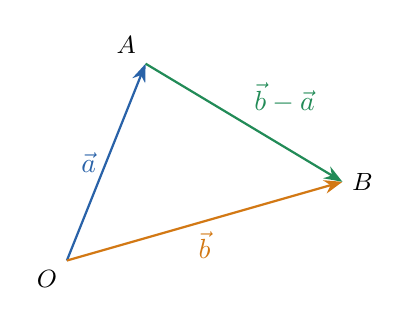
\begin{tikzpicture}[>=Stealth]
  \node[below left,font=\small] at (0,0) {$O$};
  \node[above left,font=\small] at (1,2.5) {$A$};
  \node[right,font=\small] at (3.5,1) {$B$};
  \draw[->,thick,mainblue] (0,0) -- (1,2.5) node[midway,left] {$\vec{a}$};
  \draw[->,thick,examorange] (0,0) -- (3.5,1) node[midway,below] {$\vec{b}$};
  \draw[->,thick,tipgreen] (1,2.5) -- (3.5,1) node[midway,above right] {$\vec{b}-\vec{a}$};
\end{tikzpicture}
\end{center}

% ---------- 6.3 数乘向量 ----------
\subsection*{6.3\quad 数乘向量}

\begin{knowledgebox}[数乘向量的定义与运算律]
实数 $\lambda$ 与向量 $\vec{a}$ 的乘积 $\lambda\vec{a}$ 满足：
\begin{itemize}[leftmargin=2em]
  \item $|\lambda\vec{a}| = |\lambda|\,|\vec{a}|$
  \item 当 $\lambda > 0$ 时，$\lambda\vec{a}$ 与 $\vec{a}$ 方向相同；
        当 $\lambda < 0$ 时，$\lambda\vec{a}$ 与 $\vec{a}$ 方向相反；
        当 $\lambda = 0$ 时，$\lambda\vec{a} = \vec{0}$。
\end{itemize}

\medskip
\textbf{运算律}（设 $\lambda$、$\mu$ 为实数）：
\[
\lambda(\mu\vec{a}) = (\lambda\mu)\vec{a}
\]
\[
(\lambda + \mu)\vec{a} = \lambda\vec{a} + \mu\vec{a}
\]
\[
\lambda(\vec{a} + \vec{b}) = \lambda\vec{a} + \lambda\vec{b}
\]
\end{knowledgebox}

\begin{tipbox}[向量共线定理]
向量 $\vec{b}$ 与非零向量 $\vec{a}$ 共线的充要条件是：存在唯一实数 $\lambda$，使得
\[
\vec{b} = \lambda\vec{a}
\]
\end{tipbox}

% ---------- 6.4 向量的坐标表示 ----------
\subsection*{6.4\quad 向量的坐标表示}

\begin{knowledgebox}[平面向量的坐标运算]
取 $x$ 轴、$y$ 轴上的单位向量 $\vec{i}=(1,0)$，$\vec{j}=(0,1)$，
则 $\vec{a} = x\vec{i} + y\vec{j} = (x, y)$。

\medskip
设 $\vec{a} = (a_1, a_2)$，$\vec{b} = (b_1, b_2)$，则：
\begin{enumerate}[leftmargin=2em]
  \item $\vec{a} + \vec{b} = (a_1 + b_1,\; a_2 + b_2)$
  \item $\vec{a} - \vec{b} = (a_1 - b_1,\; a_2 - b_2)$
  \item $\lambda\vec{a} = (\lambda a_1,\; \lambda a_2)$
  \item $|\vec{a}| = \sqrt{a_1^2 + a_2^2}$
  \item 若 $A(a_1,a_2)$，$B(b_1,b_2)$，则 $\overrightarrow{AB} = (b_1 - a_1,\; b_2 - a_2)$
\end{enumerate}
\end{knowledgebox}

\begin{tipbox}[中点坐标公式]
设 $A(x_1,y_1)$，$B(x_2,y_2)$，则线段 $AB$ 的中点 $M$ 的坐标为
\[
M\!\left(\frac{x_1+x_2}{2},\; \frac{y_1+y_2}{2}\right)
\]
\end{tipbox}

% ---------- 6.5 向量的数量积 ----------
\subsection*{6.5\quad 向量的数量积（点积）}

\begin{knowledgebox}[数量积的定义]
两个非零向量 $\vec{a}$ 和 $\vec{b}$ 的数量积（点积）定义为：
\[
\vec{a} \cdot \vec{b} = |\vec{a}|\,|\vec{b}|\cos\theta
\]
其中 $\theta$ 是 $\vec{a}$ 与 $\vec{b}$ 的夹角，$\theta \in [0, \pi]$。

\medskip
\textbf{坐标形式}：设 $\vec{a}=(a_1,a_2)$，$\vec{b}=(b_1,b_2)$，则
\[
\vec{a} \cdot \vec{b} = a_1 b_1 + a_2 b_2
\]
\end{knowledgebox}

\begin{knowledgebox}[数量积的性质与运算律]
\textbf{性质}：
\begin{itemize}[leftmargin=2em]
  \item $\vec{a} \cdot \vec{a} = |\vec{a}|^2$，即 $|\vec{a}| = \sqrt{\vec{a}\cdot\vec{a}}$
  \item $\cos\theta = \dfrac{\vec{a}\cdot\vec{b}}{|\vec{a}|\,|\vec{b}|}$
  \item $|\vec{a}\cdot\vec{b}| \leqslant |\vec{a}|\,|\vec{b}|$
\end{itemize}

\medskip
\textbf{运算律}：
\begin{itemize}[leftmargin=2em]
  \item $\vec{a} \cdot \vec{b} = \vec{b} \cdot \vec{a}$（交换律）
  \item $(\lambda\vec{a}) \cdot \vec{b} = \lambda(\vec{a}\cdot\vec{b})$
  \item $\vec{a}\cdot(\vec{b}+\vec{c}) = \vec{a}\cdot\vec{b} + \vec{a}\cdot\vec{c}$（分配律）
\end{itemize}

\medskip
\textbf{注意}：数量积不满足结合律，即 $(\vec{a}\cdot\vec{b})\cdot\vec{c} \neq \vec{a}\cdot(\vec{b}\cdot\vec{c})$。
\end{knowledgebox}

\begin{warnbox}[易错提醒]
\begin{itemize}[leftmargin=2em]
  \item $\vec{a}\cdot\vec{b}$ 的结果是一个\textbf{实数}，不是向量。
  \item 数量积不满足结合律：$(\vec{a}\cdot\vec{b})\vec{c}$ 是 $\vec{c}$ 的数乘，
        而 $\vec{a}(\vec{b}\cdot\vec{c})$ 是 $\vec{a}$ 的数乘，二者一般不等。
  \item 夹角 $\theta$ 的取值范围是 $[0,\pi]$，不是 $[0,2\pi)$。
\end{itemize}
\end{warnbox}

% 夹角图
\begin{center}
\begin{tikzpicture}[>=Stealth]
  \draw[->,thick,mainblue] (0,0) -- (3,0.6) node[midway,below left] {$\vec{a}$};
  \draw[->,thick,examorange] (0,0) -- (1.5,2.5) node[midway,left] {$\vec{b}$};
  \pic[draw,mainblue,angle radius=1cm,angle eccentricity=1.4,
       "$\theta$"] {angle={(3,0.6)--(0,0)--(1.5,2.5)}};
\end{tikzpicture}
\end{center}

% ---------- 6.6 向量的平行与垂直 ----------
\subsection*{6.6\quad 向量的平行与垂直}

\begin{knowledgebox}[平行与垂直的判定]
设 $\vec{a}=(a_1,a_2)$，$\vec{b}=(b_1,b_2)$，均为非零向量。

\medskip
\textbf{平行（共线）条件}：
\[
\vec{a} \parallel \vec{b} \iff a_1 b_2 - a_2 b_1 = 0
\]

\medskip
\textbf{垂直条件}：
\[
\vec{a} \perp \vec{b} \iff \vec{a}\cdot\vec{b} = 0 \iff a_1 b_1 + a_2 b_2 = 0
\]
\end{knowledgebox}

\begin{tipbox}[记忆口诀]
\textbf{平行：交叉相乘等于零}（$a_1 b_2 = a_2 b_1$）

\textbf{垂直：对应相乘加起来等于零}（$a_1 b_1 + a_2 b_2 = 0$）
\end{tipbox}

\vspace{10pt}

% ============ 第二部分：例题精讲 ============
\section*{\textcolor{examorange}{二、例题精讲}}

% 例题1：向量加减法基本运算
\begin{examplebox}[【例题1】向量加减法运算]
已知 $\vec{a}=(3,1)$，$\vec{b}=(-2,4)$，$\vec{c}=(1,-3)$，
求 $2\vec{a} - \vec{b} + 3\vec{c}$。
\end{examplebox}

\textbf{解}：
\begin{align*}
2\vec{a} - \vec{b} + 3\vec{c}
  &= 2(3,1) - (-2,4) + 3(1,-3) \\
  &= (6,2) - (-2,4) + (3,-9) \\
  &= (6+2+3,\; 2-4-9) \\
  &= (11,\;-11)
\end{align*}

\begin{tipbox}[方法总结]
向量的线性运算直接对坐标分量分别进行运算即可。
\end{tipbox}

% 例题2：向量的模
\begin{examplebox}[【例题2】求向量的模]
已知 $\vec{a}=(1,2)$，$\vec{b}=(3,-4)$，求 $|\vec{a}+\vec{b}|$ 和 $|\vec{a}-\vec{b}|$。
\end{examplebox}

\textbf{解}：
\[
\vec{a}+\vec{b} = (1+3,\; 2+(-4)) = (4,-2)
\]
\[
|\vec{a}+\vec{b}| = \sqrt{4^2+(-2)^2} = \sqrt{16+4} = \sqrt{20} = 2\sqrt{5}
\]
\[
\vec{a}-\vec{b} = (1-3,\; 2-(-4)) = (-2,6)
\]
\[
|\vec{a}-\vec{b}| = \sqrt{(-2)^2+6^2} = \sqrt{4+36} = \sqrt{40} = 2\sqrt{10}
\]

% 例题3：向量数量积与夹角
\begin{examplebox}[【例题3】数量积与夹角计算]
已知 $|\vec{a}|=3$，$|\vec{b}|=4$，$\vec{a}\cdot\vec{b}=6$，求 $\vec{a}$ 与 $\vec{b}$ 的夹角 $\theta$。
\end{examplebox}

\textbf{解}：
\[
\cos\theta = \frac{\vec{a}\cdot\vec{b}}{|\vec{a}|\,|\vec{b}|}
= \frac{6}{3\times4} = \frac{6}{12} = \frac{1}{2}
\]
因为 $\theta \in [0,\pi]$，所以 $\theta = \dfrac{\pi}{3}$（即 $60°$）。

\begin{tipbox}[方法总结]
求数量积的夹角，先用 $\cos\theta = \dfrac{\vec{a}\cdot\vec{b}}{|\vec{a}|\,|\vec{b}|}$ 求出余弦值，
再结合 $\theta \in [0,\pi]$ 确定角度。
\end{tipbox}

% 例题4：平行条件
\begin{examplebox}[【例题4】向量平行的判定]
已知 $\vec{a}=(2,-3)$，$\vec{b}=(x,6)$，若 $\vec{a} \parallel \vec{b}$，求 $x$ 的值。
\end{examplebox}

\textbf{解}：

$\vec{a} \parallel \vec{b}$ 的条件为 $a_1 b_2 - a_2 b_1 = 0$，代入得：
\[
2 \times 6 - (-3) \times x = 0
\]
\[
12 + 3x = 0
\]
\[
x = -4
\]

验证：$\vec{b}=(-4,6)=-2(2,-3)=-2\vec{a}$，确实平行。

% 例题5：垂直条件
\begin{examplebox}[【例题5】向量垂直的判定]
已知 $\vec{a}=(1,m)$，$\vec{b}=(2m, -2)$，若 $\vec{a} \perp \vec{b}$，求 $m$ 的值。
\end{examplebox}

\textbf{解}：

$\vec{a} \perp \vec{b}$ 的条件为 $\vec{a}\cdot\vec{b} = 0$，即：
\[
1 \times 2m + m \times (-2) = 0
\]
\[
2m - 2m = 0
\]
\[
0 = 0
\]

此式对任意实数 $m$ 恒成立。

但需注意：$\vec{a} \perp \vec{b}$ 要求 $\vec{a}$ 和 $\vec{b}$ 都是非零向量。
$\vec{a}=\vec{0}$ 当 $1=0$ 不成立；$\vec{b}=\vec{0}$ 当 $2m=0$ 且 $-2=0$ 也不成立。

因此对任意实数 $m$，均有 $\vec{a} \perp \vec{b}$。

\begin{warnbox}[易错提醒]
判断垂直时，除了验证 $\vec{a}\cdot\vec{b}=0$ 外，还需确认两个向量都是非零向量。
\end{warnbox}

% 例题6：向量的模与数量积综合
\begin{examplebox}[【例题6】利用数量积求模]
已知 $|\vec{a}|=2$，$|\vec{b}|=3$，$\vec{a}$ 与 $\vec{b}$ 的夹角为 $120°$，求 $|\vec{a}+\vec{b}|$。
\end{examplebox}

\textbf{解}：

先求 $\vec{a}\cdot\vec{b}$：
\[
\vec{a}\cdot\vec{b} = |\vec{a}|\,|\vec{b}|\cos 120° = 2 \times 3 \times \left(-\frac{1}{2}\right) = -3
\]

利用 $|\vec{a}+\vec{b}|^2 = (\vec{a}+\vec{b})\cdot(\vec{a}+\vec{b})$：
\begin{align*}
|\vec{a}+\vec{b}|^2
  &= \vec{a}\cdot\vec{a} + 2\vec{a}\cdot\vec{b} + \vec{b}\cdot\vec{b} \\
  &= |\vec{a}|^2 + 2\vec{a}\cdot\vec{b} + |\vec{b}|^2 \\
  &= 4 + 2\times(-3) + 9 \\
  &= 4 - 6 + 9 = 7
\end{align*}
\[
|\vec{a}+\vec{b}| = \sqrt{7}
\]

\begin{tipbox}[方法总结]
求 $|\vec{a}\pm\vec{b}|$ 时，利用 $|\vec{a}\pm\vec{b}|^2 = |\vec{a}|^2 \pm 2\vec{a}\cdot\vec{b} + |\vec{b}|^2$，
先求出数量积，再开方。
\end{tipbox}

% 例题7：三点共线问题
\begin{examplebox}[【例题7】三点共线的证明]
已知 $A(1,2)$，$B(3,4)$，$C(5,6)$，证明 $A$、$B$、$C$ 三点共线。
\end{examplebox}

\textbf{解}：
\[
\overrightarrow{AB} = (3-1,\; 4-2) = (2, 2)
\]
\[
\overrightarrow{AC} = (5-1,\; 6-2) = (4, 4)
\]

因为 $\overrightarrow{AC} = 2\overrightarrow{AB}$，即 $\overrightarrow{AC}$ 与 $\overrightarrow{AB}$ 共线，
且它们有公共起点 $A$，所以 $A$、$B$、$C$ 三点共线。

\begin{tipbox}[方法总结]
三点共线的证明方法：设三点为 $A$、$B$、$C$，
只需证明 $\overrightarrow{AB}$ 与 $\overrightarrow{AC}$（或 $\overrightarrow{BC}$）共线，
即 $\overrightarrow{AB} = \lambda \overrightarrow{AC}$，或 $x_1 y_2 - x_2 y_1 = 0$。
\end{tipbox}

% 例题8：综合题——向量垂直与坐标
\begin{examplebox}[【例题8】综合题——向量运算与垂直判定]
已知 $\vec{a}=(2,1)$，$\vec{b}=(1,3)$，设 $\vec{c} = \vec{a} + t\vec{b}$（$t \in \mathbb{R}$），当 $t$ 为何值时：
\begin{enumerate}[label=(\arabic*)]
  \item $|\vec{c}|$ 最小？最小值是多少？
  \item 此时 $\vec{c}$ 与 $\vec{b}$ 是否垂直？
\end{enumerate}
\end{examplebox}

\textbf{解}：

（1）$\vec{c} = \vec{a} + t\vec{b} = (2,1) + t(1,3) = (2+t,\; 1+3t)$

\begin{align*}
|\vec{c}|^2 &= (2+t)^2 + (1+3t)^2 \\
  &= 4 + 4t + t^2 + 1 + 6t + 9t^2 \\
  &= 10t^2 + 10t + 5 \\
  &= 10\!\left(t^2 + t\right) + 5 \\
  &= 10\!\left(t + \frac{1}{2}\right)^2 - \frac{10}{4} + 5 \\
  &= 10\!\left(t + \frac{1}{2}\right)^2 + \frac{5}{2}
\end{align*}

当 $t = -\dfrac{1}{2}$ 时，$|\vec{c}|^2$ 取最小值 $\dfrac{5}{2}$，
此时 $|\vec{c}|_{\min} = \sqrt{\dfrac{5}{2}} = \dfrac{\sqrt{10}}{2}$。

（2）当 $t=-\dfrac{1}{2}$ 时，$\vec{c} = \left(2-\dfrac{1}{2},\; 1-\dfrac{3}{2}\right) = \left(\dfrac{3}{2},\; -\dfrac{1}{2}\right)$

\[
\vec{c}\cdot\vec{b} = \frac{3}{2}\times 1 + \left(-\frac{1}{2}\right)\times 3 = \frac{3}{2} - \frac{3}{2} = 0
\]

因为 $\vec{c}\cdot\vec{b} = 0$，且 $\vec{c} \neq \vec{0}$，$\vec{b} \neq \vec{0}$，
所以此时 $\vec{c} \perp \vec{b}$。

\begin{tipbox}[方法总结]
求含参数向量模的最值，常用配方法或二次函数求最值的方法。求出参数后代入验证其他条件。
\end{tipbox}

% 例题9：向量夹角的坐标公式
\begin{examplebox}[【例题9】用坐标求向量夹角]
已知 $\vec{a}=(1,\sqrt{3})$，$\vec{b}=(2,0)$，求 $\vec{a}$ 与 $\vec{b}$ 的夹角。
\end{examplebox}

\textbf{解}：
\[
\vec{a}\cdot\vec{b} = 1\times 2 + \sqrt{3}\times 0 = 2
\]
\[
|\vec{a}| = \sqrt{1+3} = 2, \quad |\vec{b}| = \sqrt{4+0} = 2
\]
\[
\cos\theta = \frac{\vec{a}\cdot\vec{b}}{|\vec{a}|\,|\vec{b}|} = \frac{2}{2\times 2} = \frac{1}{2}
\]
因为 $\theta \in [0,\pi]$，所以 $\theta = \dfrac{\pi}{3}$（即 $60°$）。

% 例题10：向量与三角形
\begin{examplebox}[【例题10】向量法判断三角形的形状]
在 $\triangle ABC$ 中，已知 $\overrightarrow{AB}=(2,1)$，$\overrightarrow{AC}=(1,k)$，
若 $\triangle ABC$ 为直角三角形且 $\angle A = 90°$，求 $k$ 的值。
\end{examplebox}

\textbf{解}：

$\angle A = 90°$ 即 $\overrightarrow{AB} \perp \overrightarrow{AC}$，所以：
\[
\overrightarrow{AB}\cdot\overrightarrow{AC} = 0
\]
\[
2\times 1 + 1\times k = 0
\]
\[
2 + k = 0
\]
\[
k = -2
\]

\begin{tipbox}[方法总结]
用向量方法处理几何问题时，将角度条件转化为向量的数量积为零（垂直）或共线条件。
\end{tipbox}

\vspace{10pt}

% ============ 第三部分：应用题 ============
\section*{\textcolor{apppurple}{三、应用题}}

% 应用1：物理中的力的合成
\begin{appbox}[【应用1】力的合成]
两个力 $\vec{F_1}$ 和 $\vec{F_2}$ 作用在同一物体上。已知 $|\vec{F_1}|=30\;\text{N}$，
$|\vec{F_2}|=40\;\text{N}$，两力夹角为 $90°$。求合力 $\vec{F}=\vec{F_1}+\vec{F_2}$ 的大小。
\end{appbox}

\textbf{解}：

建立坐标系，设 $\vec{F_1}=(30,0)$，$\vec{F_2}=(0,40)$，则
\[
\vec{F} = \vec{F_1}+\vec{F_2} = (30,40)
\]
\[
|\vec{F}| = \sqrt{30^2+40^2} = \sqrt{900+1600} = \sqrt{2500} = 50 \;\text{N}
\]

\begin{center}
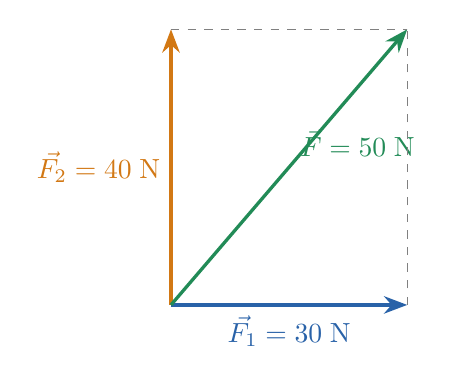
\begin{tikzpicture}[>=Stealth]
  \draw[->,very thick,mainblue] (0,0) -- (3,0) node[midway,below] {$\vec{F_1}=30\;\text{N}$};
  \draw[->,very thick,examorange] (0,0) -- (0,3.5) node[midway,left] {$\vec{F_2}=40\;\text{N}$};
  \draw[->,very thick,tipgreen] (0,0) -- (3,3.5) node[midway,above right] {$\vec{F}=50\;\text{N}$};
  \draw[dashed,gray] (3,0) -- (3,3.5);
  \draw[dashed,gray] (0,3.5) -- (3,3.5);
\end{tikzpicture}
\end{center}

合力大小为 $50\;\text{N}$。

% 应用2：速度合成
\begin{appbox}[【应用2】船过河问题]
一条船在静水中的速度为 $4\;\text{m/s}$，河水流速为 $3\;\text{m/s}$，河宽 $d=200\;\text{m}$。
\begin{enumerate}[label=(\arabic*)]
  \item 若要使船垂直于河岸到达对岸，船头应朝哪个方向？渡河时间是多少？
  \item 若船头垂直于河岸方向行驶，实际到达对岸时偏移了多少？
\end{enumerate}
\end{appbox}

\textbf{解}：

（1）设水流方向为 $x$ 轴正方向，垂直于河岸向对岸为 $y$ 轴正方向。

水流速度 $\vec{v_水}=(3,0)$，设船在静水中速度方向与河岸夹角为 $\alpha$，
则 $\vec{v_船}=(4\cos\alpha,\; 4\sin\alpha)$。

合速度 $\vec{v}=\vec{v_船}+\vec{v_水}=(3+4\cos\alpha,\; 4\sin\alpha)$。

要垂直过河，水平分量为零：
\[
3 + 4\cos\alpha = 0 \implies \cos\alpha = -\frac{3}{4}
\]
\[
\sin\alpha = \sqrt{1-\frac{9}{16}} = \frac{\sqrt{7}}{4}
\]
此时船头应朝上游偏转，$\alpha = \pi - \arccos\dfrac{3}{4}$。

合速度竖直分量 $v_y = 4\sin\alpha = 4 \times \dfrac{\sqrt{7}}{4} = \sqrt{7}\;\text{m/s}$

渡河时间 $t = \dfrac{d}{v_y} = \dfrac{200}{\sqrt{7}} = \dfrac{200\sqrt{7}}{7} \approx 75.6\;\text{s}$。

（2）船头垂直河岸时，$\alpha=90°$，$\vec{v_船}=(0,4)$，$\vec{v}=(3,4)$。

渡河时间 $t = \dfrac{200}{4} = 50\;\text{s}$。

水平偏移量 $\Delta x = 3 \times 50 = 150\;\text{m}$。

\begin{center}
\begin{tikzpicture}[>=Stealth]
  \draw[->,thick,mainblue] (0,0) -- (3,0) node[midway,below] {$\vec{v_水}$};
  \draw[->,thick,examorange] (0,0) -- (0,2.5) node[midway,left] {$\vec{v_船}$};
  \draw[->,very thick,tipgreen] (0,0) -- (3,2.5) node[midway,above right] {$\vec{v}$};
  \draw[dashed,gray] (3,0) -- (3,2.5) -- (0,2.5);
  \node[font=\small] at (4.2,1.25) {偏移};
  \draw[->,gray] (3.5,1.25) -- (3.2,1.25);
\end{tikzpicture}
\end{center}

% 应用3：几何证明
\begin{appbox}[【应用3】向量法证明几何定理]
用向量法证明：平行四边形的对角线互相平分。
\end{appbox}

\textbf{证明}：

设平行四边形 $ABCD$，设 $A$ 为原点。

令 $\overrightarrow{AB}=\vec{a}$，$\overrightarrow{AD}=\vec{b}$。

则：
\[
\overrightarrow{AC} = \overrightarrow{AB} + \overrightarrow{BC} = \vec{a} + \vec{b}
\]
\[
\overrightarrow{DB} = \overrightarrow{AB} - \overrightarrow{AD} = \vec{a} - \vec{b}
\]

设 $AC$ 的中点为 $M_1$，则
\[
\overrightarrow{AM_1} = \frac{1}{2}\overrightarrow{AC} = \frac{1}{2}(\vec{a}+\vec{b})
\]

设 $DB$ 的中点为 $M_2$，则
\[
\overrightarrow{AM_2} = \overrightarrow{AD} + \frac{1}{2}\overrightarrow{DB}
= \vec{b} + \frac{1}{2}(\vec{a}-\vec{b}) = \frac{1}{2}\vec{a} + \frac{1}{2}\vec{b}
= \frac{1}{2}(\vec{a}+\vec{b})
\]

因为 $\overrightarrow{AM_1} = \overrightarrow{AM_2}$，所以 $M_1$ 与 $M_2$ 重合，
即对角线 $AC$ 和 $BD$ 互相平分。$\blacksquare$

\begin{center}
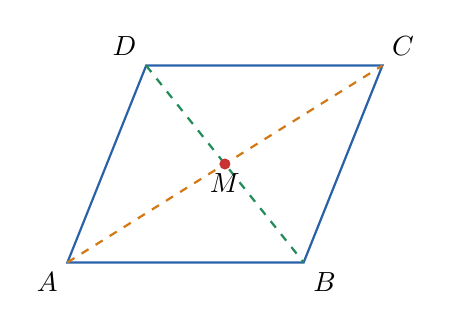
\begin{tikzpicture}[>=Stealth]
  \coordinate[label=below left:$A$] (A) at (0,0);
  \coordinate[label=below right:$B$] (B) at (3,0);
  \coordinate[label=above right:$C$] (C) at (4,2.5);
  \coordinate[label=above left:$D$] (D) at (1,2.5);
  \draw[thick,mainblue] (A)--(B)--(C)--(D)--cycle;
  \draw[thick,examorange,dashed] (A)--(C);
  \draw[thick,tipgreen,dashed] (D)--(B);
  \coordinate[label=below:$M$] (M) at ($0.5*(A)+0.5*(C)$);
  \fill[warnred] (M) circle(2pt);
\end{tikzpicture}
\end{center}

% 应用4：导航问题
\begin{appbox}[【应用4】导航与位移]
一架飞机从 $A$ 地出发，先向北偏东 $60°$ 方向飞行 $200\;\text{km}$ 到达 $B$ 地，
再从 $B$ 地向北偏西 $30°$ 方向飞行 $100\;\text{km}$ 到达 $C$ 地。
求 $A$、$C$ 两地的距离（精确到 $1\;\text{km}$）。
\end{appbox}

\textbf{解}：

建立坐标系：以 $A$ 为原点，正东为 $x$ 轴正方向，正北为 $y$ 轴正方向。

$AB$ 段：北偏东 $60°$，即从正北向东偏 $60°$，对应方向角 $90°-60°=30°$（从 $x$ 轴正方向逆时针）。
\[
\overrightarrow{AB} = (200\cos 30°,\; 200\sin 30°) = (100\sqrt{3},\; 100)
\]

$BC$ 段：北偏西 $30°$，即从正北向西偏 $30°$，对应方向角 $90°+30°=120°$。
\[
\overrightarrow{BC} = (100\cos 120°,\; 100\sin 120°) = (-50,\; 50\sqrt{3})
\]

\[
\overrightarrow{AC} = \overrightarrow{AB} + \overrightarrow{BC}
= (100\sqrt{3}-50,\; 100+50\sqrt{3})
\]
\[
= (100\sqrt{3}-50,\; 100+50\sqrt{3})
\approx (123.21,\; 186.60)
\]
\[
|\overrightarrow{AC}| = \sqrt{(100\sqrt{3}-50)^2 + (100+50\sqrt{3})^2}
\]

展开计算：
\begin{align*}
&(100\sqrt{3}-50)^2 = 30000 - 10000\sqrt{3} + 2500 = 32500 - 10000\sqrt{3} \\
&(100+50\sqrt{3})^2 = 10000 + 10000\sqrt{3} + 7500 = 17500 + 10000\sqrt{3}
\end{align*}
\[
|\overrightarrow{AC}|^2 = 32500 - 10000\sqrt{3} + 17500 + 10000\sqrt{3} = 50000
\]
\[
|\overrightarrow{AC}| = \sqrt{50000} = 100\sqrt{5} \approx 224\;\text{km}
\]

$A$、$C$ 两地的距离约为 $224\;\text{km}$。

\vspace{10pt}

% ============ 第四部分：课堂练习 ============
\section*{\textcolor{tipgreen}{四、课堂练习}}

\begin{enumerate}[label=\textbf{\arabic*.}, leftmargin=2em]
  \item 已知 $\vec{a}=(3,-1)$，$\vec{b}=(-1,2)$，求 $3\vec{a}+2\vec{b}$ 和 $\vec{a}-3\vec{b}$。

  \item 已知 $\vec{a}=(4,3)$，求 $|\vec{a}|$ 和与 $\vec{a}$ 同方向的单位向量 $\vec{e}$。

  \item 已知 $|\vec{a}|=5$，$|\vec{b}|=8$，$\vec{a}$ 与 $\vec{b}$ 的夹角为 $60°$，求 $\vec{a}\cdot\vec{b}$。

  \item 已知 $\vec{a}=(2,-1)$，$\vec{b}=(4,8)$，判断 $\vec{a}$ 与 $\vec{b}$ 的位置关系（平行、垂直或既不平行也不垂直）。

  \item 已知 $\vec{a}=(1,2)$，$\vec{b}=(3,-4)$，$\vec{c}=\vec{a}+\lambda\vec{b}$，
        若 $\vec{c} \perp \vec{a}$，求 $\lambda$ 的值。

  \item 已知 $A(2,1)$，$B(-1,3)$，$C(0,-1)$，求 $\overrightarrow{AB}\cdot\overrightarrow{AC}$ 和 $\angle BAC$ 的度数。

  \item 已知 $|\vec{a}|=1$，$|\vec{b}|=2$，$|\vec{a}-\vec{b}|=\sqrt{3}$，求 $\vec{a}\cdot\vec{b}$。
\end{enumerate}

\begin{knowledgebox}[参考答案]
\begin{enumerate}[label=\textbf{\arabic*.}, leftmargin=2em]
  \item $3\vec{a}+2\vec{b} = 3(3,-1)+2(-1,2) = (9,-3)+(-2,4) = (7,1)$

        $\vec{a}-3\vec{b} = (3,-1)-3(-1,2) = (3,-1)-(-3,6) = (6,-7)$

  \item $|\vec{a}| = \sqrt{16+9} = 5$；

        单位向量 $\vec{e} = \dfrac{\vec{a}}{|\vec{a}|} = \left(\dfrac{4}{5},\; \dfrac{3}{5}\right)$

  \item $\vec{a}\cdot\vec{b} = 5\times 8\times\cos 60° = 40\times\dfrac{1}{2} = 20$

  \item $\vec{a}\cdot\vec{b} = 2\times 4 + (-1)\times 8 = 8-8 = 0$

        因为 $\vec{a}\cdot\vec{b}=0$ 且两个向量均为非零向量，所以 $\vec{a}\perp\vec{b}$，即 $\vec{a}$ 与 $\vec{b}$ 垂直。

  \item $\vec{c} = (1+3\lambda,\; 2-4\lambda)$

        $\vec{c}\perp\vec{a}$ 要求 $\vec{c}\cdot\vec{a}=0$：
        $(1+3\lambda)\times 1 + (2-4\lambda)\times 2 = 0$

        $1+3\lambda + 4-8\lambda = 0 \implies 5-5\lambda = 0 \implies \lambda = 1$

  \item $\overrightarrow{AB}=(-3,2)$，$\overrightarrow{AC}=(-2,-2)$

        $\overrightarrow{AB}\cdot\overrightarrow{AC} = (-3)\times(-2)+2\times(-2) = 6-4 = 2$

        $|\overrightarrow{AB}|=\sqrt{9+4}=\sqrt{13}$，$|\overrightarrow{AC}|=\sqrt{4+4}=2\sqrt{2}$

        $\cos\angle BAC = \dfrac{2}{\sqrt{13}\times 2\sqrt{2}} = \dfrac{2}{2\sqrt{26}} = \dfrac{1}{\sqrt{26}}$

        $\angle BAC = \arccos\dfrac{1}{\sqrt{26}} \approx 78.7°$

  \item $|\vec{a}-\vec{b}|^2 = (\vec{a}-\vec{b})\cdot(\vec{a}-\vec{b})
        = |\vec{a}|^2 - 2\vec{a}\cdot\vec{b} + |\vec{b}|^2$

        $3 = 1 - 2\vec{a}\cdot\vec{b} + 4 \implies 2\vec{a}\cdot\vec{b} = 2 \implies \vec{a}\cdot\vec{b} = 1$
\end{enumerate}
\end{knowledgebox}

\vfill
\begin{center}
\small\textcolor{gray}{本讲义仅供教学参考，例题可根据学生水平调整难度。}
\end{center}

\end{document}
